% !TEX root = ../thesis-example.tex
\chapter{Concepts}
\label{sec:concepts}

\section{Definitions}
\label{sec:concepts:defs}

In the following definitions are given to reason about semantics of implementations of a TeSSLa runtime.
A TeSSLa specification gives a number of transformations over Streams and a subset of the generated streams as outputs.

\subsection{Streams}
\label{sec:concepts:defs:streams}

There are two kind of streams: Signals, which carry values at all times and EventStreams, which only hold values at specific times.
EventStreams can be described by a sequence of Events.
Signals can be described by a sequence of changes, where a change notes that the value of a Signal changed at a specific timestamp.
The only difference between a Signal and an EventStreams is that Signals always have a value while an EventStream may return \(\bot\), which denotes, that no event happened at that time.
Because the similarity of Signals and EventStreams in the following we will mainly reason about EventStreams, but most things can also be applied to Signals.

Formally a stream \(\sigma\) is defined as a Sequence of Events, the Set of all Streams \(\Sigma\) is defined as all possible finite sequences of Events \(\Sigma = \{\sigma | \sigma \in E^* \}\)
An input Stream \(\sigma_i\) is a stream consisting of only input events, the set of all input Streams is \(\Sigma_i = \{\sigma_i | \sigma_i \in E_i^*\}\).
Output and internal Streams are defined analogous.

Furthermore Streams hold the timestamp to which they have progressed, which can be equal or greater than the timestamp of the last Event happened on them.

\subsection{Events}
\label{sec:concepts:defs:events}

Streams consists of Events (or changes, which can be modeled the same as events).
There are three Types of Events: input, output and internal Events.

The Set of all Events is denoted as \(E\).
Each event carries a value, which can be \emph{nothing} or a value of a Type (types are formally defined in the TeSSLa speicification but aren't important for this thesis), a timestamp and the channel it's perceived on (e.g.\ a function call of a specific function or the name of an output stream).

\(E_i \subset E\) is the Set of all input events, their channel corresponds to a specific trace.
\(E_o \subset E\) is the Set of all output events, their channel is specified by an output name of the TeSSLa specification.
\(E_n \subset E\) is the Set of all internal events.
Internal events are mostly an implementation detail, which denote steps of computation inside the runtime.
The channel of internal events is implicitly given by the node that produces the stream of the Event.
Note that \(E_i, E_o, E_n\) are pairwise disjoint and \(E_i \cup E_o \cup E_n = E\).

\subsection{Functions}
\label{sec:concepts:defs:functions}

A TeSSLa specification consists of functions.
Functions generate new Streams by applying operation on other stream.
TeSSLa itself defines a syntax to write a specification, a set of types and a standard library of functions, but an implementation is free to choose the functions it supports.

An example function is \(add(S_D,S_D) \rightarrow S_D\): It takes two Signals, which have to hold values of some numerical type, and produces a signal which holds values of the same type.
The produced stream can either be assigned to a named identifier (think: a variable) or directly be given to another function (function composition).

Functions can be divided into three categories: pure, unpure and timing.
Pure Functions, also called stateless, are evaluated only on the values their inputs have at the timestamp they are evaluated, therefore they don't have to \emph{remember} anything about earlier events.
Unpure, or stateful, Functions are evaluatet with additional, stored information, which they can mutate.
E.g.\ a Function \emph{eventCount} has to \emph{remember} how many events already happened on it's input stream and increment that counter on every new event.
Timing Functions are evaluated not only on the value of Events but also on their timestamp and can also manipulate it:
While non timing functions will consume events at a specific timestamp and emit an event with that timestamp, timing functions can emit Events with a different timestamp.

Timing Functions complicate the reasoning about schedules and causality and therefore aren't included in Section~\ref{sec:concepts:behaviour_without_timing}.
In Section~\ref{sec:concepts:behaviour_with_timing} the conclusions of earlier sections will be extended to include timing functions.


\subsection{Nodes}
\label{sec:concepts:defs:nodes}

Nodes are the atomic unit of computation for the evaluation of a TeSSLa specification.
A Node implements a single Function, e.g.:\ there is an \emph{AddNode} which takes two input Signals and produces a new Signal.
Therefore a Node is the concrete implementation of a function in a runtime for TeSSLa specifications.
Each Node has a set of inputs, which are either input or internal Streams, and one output, which is either an internal or an output Stream.


Nodes use a FIFO queue, provided by the Erlang plattform, to process new received Events in multiple steps:

\begin{enumerate}
  \item Add the new Event to the inputs
  \item Check if a new output Event can be produced (see Section~\ref{sec:concepts:defs:nodes:processable})
  \item If so, compute all timestamps, where new Events might be computed and
    \begin{enumerate}
      \item Compute the Events, add them to the History as new outputs
      \item Distribute the updated output to all successors
    \end{enumerate}
  \item Else wait for another input
\end{enumerate}

\subsubsection{Determination of processable Events}
\label{sec:concepts:defs:nodes:processable}

Based on the asynchronous nature of Nodes, Events from different Streams can be received out of order.
E.g.\ if a Node C is a child of Node A and B, it can receive Events from Node A at timestamps \(t_1, t_2, t_3, t_4\)
before receiving an event with timestamp \(t_1\) from Node B.
Therefore a Node can not compute it's output upto a timestamp unless it has informations from all predecessors that they did progress to that timestamp.
When Node C receives the first four Events from Node A, it will only add them to it's inputs but won't compute an output.
When it finally receives the first Event from Node B it can compute all Events upto \(t_1\).
To do so it will compute \emph{change timestamps}: The union of all timestamps where an Event occured on any input between the timestamp of the last generated output and the minimal progress of all inputs.

To see why this is necessary lets assume that Node C will receive a new Event from Node B with timestamp \(t_4\):
All inputs have progressed to \(t_4\), but on the stream from Node A there are changes between \(t_1\) (where the last output was generated) and \(t_4\),
therefore the \emph{change timestamps} are \(t_2, t_3, t_4\) and the Node will have to compute it's output based on the values of the streams at that timestamps.

\subsection{TeSSLa Evaluation Engine}
\label{sec:concepts:def:model}

Because Functions in TeSSLa specifications itself depend on other Functions, and these dependencies have to be circle free,
the specification can be represented as a DAG@.
This DAG can be directly translated into an evaluation Model for that specification: The Nodes of the DAGs are Nodes representing the functions and the Edges are the input and output Streams between the Nodes.

A Node in the DAG is called \emph{ready} when it has at least one event buffered on all of it's inputs, meaning it is able to perform a computation and produce a new output.

A Node in the DAG is called independent of another Node, if it is no descendant of that Node.
This means the Node doesn't depend on the Events emitted by the other Node.

To evaluate a specification over Traces, the Evaluation Engine has process the Events that were traced.
To do so the Nodes have to run their computations until no more Events are present (or the specification found an error in the trace).
This leads to the question in which order Nodes should be scheduled to perform their computation.
While some schedules are simply not rational (think of unfairness and causality) there are many different schedules that are feasible.
It has to be prooven that a chosen schedule produces the correct conclusions for a specification, else the Evaluation Engine is not valid.

In this Thesis it is shown that multiple schedules will lead to the same conclusions and therefore an implementation of an Evaluation Engine is free to choose between them.

\subsection{State}
\label{sec:concepts:def:state}

All TeSSLa evaluation Engines have to hold a State, which encodes information necessary to continue the evaluation.
The State of a whole Evaluation Engine is made up of the States of it's Nodes.

Each Node has a State that can hold arbitrary data used for computation.
One part of the State of every Node is the History of a Node, which holds all Events received from it's parents, called it's inputs, and all produced Events of the Node, called it's output.
Other information stored in the State may be the number of Events seen by an \emph{eventCountNode} which is incremented everytime the Node consumes a new input.

Formally the State of a Node is a tuple of some arbitrary information, the inputs (a set of internal and input Streams) and the output (an internal or an output Stream).
Everytime a Node is scheduled it changes it State by:

\begin{itemize}
  \item Updating it's inputs
  \item updating it's output
  \item optionally updating its arbitrary information
\end{itemize}

\subsection{Transitions}
\label{sec:concepts:def:transitions}

A Transition describes what happens when the evaluation engine switches State by performing a Step:
The consumption of one Event from each input of a Node and the computation of a new output from that Node.
Formally a Transition maps a sequence of Events to one Event.
The empty transition, meaning no input was consumed or produced, is labeled with \(\lambda\).

\subsection{Run}
\label{sec:concepts:def:run}

A Run of an Evaluation Engine is a sequence of Transitions and States.
The first element of the sequence is the empty transition and the initial state of the evaluation engine.
It is a representation of the steps the Engine takes to evaluate a specification over streams.
The run \(\langle (\lambda, s_0), (\tau_1, s_1) \rangle\) means, that the Engine was in it's initial State, took the transition \(\tau_1\) and thereby reached the state \(s_1\).

\section{Behaviour of different schedules without timing functions}
\label{sec:concepts:behaviour_without_timing}

For a first step we specify and compare behaviours of different approaches to evaluate TeSSLa specifications without timing formulas,
meaning that only functions, which manipulate values or the presence of events, but not the timestamp of them, are used.
This leads to behaviours that can be easily reason about, as seen in the next sections.

All Evaluation Engines compute Events in steps.
At each step a Node is scheduled to perform it's specific operation, therefore one of the following things can happen in each step.

\begin{itemize}
  \item An input Event can be consumed by a source in the DAG, which generates an internal event that is propagated to it's children
  \item An internal Node which has at least one new input buffered on all of its input queues can perform
    it's computation and generate a new internal event, which is propagated to the children of that node, which therefore can compute in the next step.
  \item An output node, which has at least one new input buffered on its input queue, can produce a new output.
\end{itemize}

Evaluation Engines are free in the way they are scheduling their Nodes.
In the following we will classify Evaluation Engines by their scheduling approaches.

\subsection{Synchronous Evaluation Engines}
\label{sec:concepts:behaviour_without_timing:synchronous}

An synchronous Evaluation Engine is one that has a fixed schedule, build like this:
Number all Nodes in a reversed topological order, then always schedule the Node with the lowest number that is ready.
Obviously for many DAGs there is no unique reversed topological order, therefore one can be chosen by the evaluation engine.

This schedule ensures that no Node is scheduled which has a successor that can be scheduled, therefore Events are \emph{pushed} through the DAG towards an output Node as fast as possible.

A synchronous Evaluation Engine is considered as the \emph{Source of Truth}:
Any other Evaluation Engine has to be equal to one, else it is not a valid evaluation engine.

\begin{figure}
  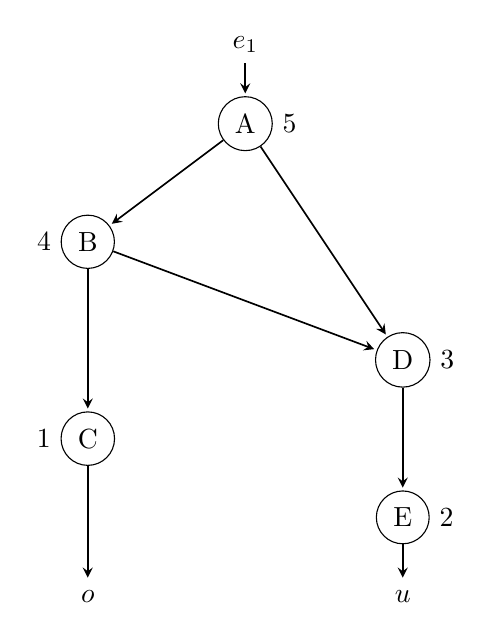
\begin{tikzpicture}
    [pre/.style={<-,shorten <=1pt,>=stealth,semithick}]
    \node (S) at (2,5) {\(e_1\)};
    \node [shape=circle,draw=black] (A) [label=right:5] at (2, 4) {A}
      edge [pre] (S);
    \node [shape=circle,draw=black] (B) [label=left:4] at (0,2.5) {B}
      edge [pre] (A);
    \node [shape=circle,draw=black] (C) [label=left:1] at (0,0) {C}
      edge [pre] (B);
    \node [shape=circle,draw=black] (D) [label=right:3] at (4,1) {D}
      edge [pre] (A)
      edge [pre] (B);
    \node [shape=circle,draw=black] (E) [label=right:2] at (4,-1) {E}
      edge [pre] (D);
    \node (o1) at (0,-2) {\(o\)} edge [pre] (C);
    \node (o2) at (4,-2) {\(u\)} edge [pre] (E);
  \end{tikzpicture}
  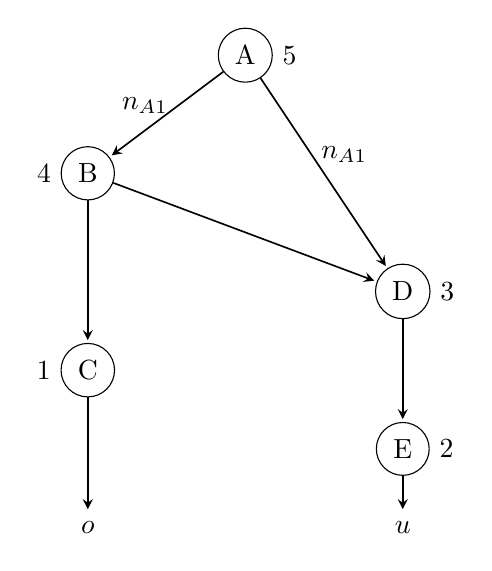
\begin{tikzpicture}
    [pre/.style={<-,shorten <=1pt,>=stealth,semithick}]
    \node [shape=circle,draw=black] (A) [label=right:5] at (2, 4) {A};
    \node [shape=circle,draw=black] (B) [label=left:4] at (0,2.5) {B}
      edge [pre] node[align=left,left,pos=0.6] {\(n_{A1}\)} (A);
    \node [shape=circle,draw=black] (C) [label=left:1] at (0,0) {C}
      edge [pre] (B);
    \node [shape=circle,draw=black] (D) [label=right:3] at (4,1) {D}
      edge [pre] node[align=right,right,pos=0.6] {\(n_{A1}\)} (A)
      edge [pre] (B);
    \node [shape=circle,draw=black] (E) [label=right:2] at (4,-1) {E}
      edge [pre] (D);
    \node (o1) at (0,-2) {\(o\)} edge [pre] (C);
    \node (o2) at (4,-2) {\(u\)} edge [pre] (E);
  \end{tikzpicture}
  \caption{Visualization of a simple asynchronous system with a reversed topological order.}
\label{fig:chap3:sec_sync:visual_dag}
\end{figure}
% The behaviour for a single input can be described by two functions:


Figure~\ref{fig:chap3:sec_sync:visual_dag} visualizes a synchronous System.
It shows two DAG representations of an evaluation Engine  where the Nodes A to E are labeled in a reversed topological order and \(o\) and \(u\) represents the output channels with that name.
The left System is in it's initial State and an input event \(e_1\) is ready to be consumed.
When a Node is chosen to compute by the scheduler, only Node A is ready, therefore it is scheduled.
The right system is the representation of the next step: Node A has consumed the external event and produced an internal event \(n_{A1}\) which is propagated to all it's children: Node B and D.
In the next step Node B would be scheduled, because it has the lowest number of any node that can compute (actually it's the only node that can compute at all, because D has to wait for the event from B).
After B was scheduled, it would have produced the internal Event \(n_{B1}\) which would then be distributed to Nodes C and D.

The complete run of the synchronous Engine for one Input is the following, where the States are not further defined:

\begin{align*}
  \langle
    (\lambda,                                    s_0),
    (\langle n_{A1}         \rangle\rightarrow n_{B1},  s_1),
    (\langle n_{B1}         \rangle\rightarrow o_1,     s_2),\\
    (\langle n_{A1}, n_{B1} \rangle\rightarrow n_{D1},  s_3),
    (\langle n_{D1}         \rangle\rightarrow u_1,     s_4)
  \rangle
\end{align*}

If there were more than one input event, at this point Node A would be scheduled again.
It would consume the next input and the following nodes would be scheduled in the same order as before, extending the run in an obvious way.

\subsection{Asynchronous evaluation}
\label{sec:concepts:behaviour_without_timing:async}

An asynchronous evaluation Engine one with a fair, but not fixed schedule.

In contrast to the synchronous evaluation Engine it has no fixed schedule, the only requirement is that the schedule is fair.
Therefore predecessors of ready Nodes can perform multiple computations before their children are scheduled and Events are not \emph{pushed} through the DAG as fast as possible.
\todo{later}

\section{Equalitys of different schedules without timing functions}
\label{sec:concepts:equalitys_without_timing}

Based on the described behaviours of the approaches we now can proof the equality of different Schedules for an Engine.
Two Engines for a TeSSLa specification are equal, if they produce the same outputs for the same inputs.
Because the consumed inputs and produced outputs can be reconstructed from a Run, we can show equality by showing that Runs are equal.

Two Runs are assumed to be equal if the State of their last elements are equal.
Because all generated Events are saved in the State of an Engine, if two Runs have the same State in their last element they did produce the same outputs.


As already stated in Section~\ref{sec:concepts:behaviour_without_timing:synchronous} a synchronous evaluation Engine is regarded as the source of truth, therefore all other kinds of evaluation Engines have to be equal to one.

The Equality is shown in two steps: First in Section~\ref{sec:concepts:equalitys_without_timing:synchronous}it is shown, that all possible synchronous Engines for a specification are equal, so there is only one true Evaluation.
Afterwards in Section~\ref{sec:concepts:equalitys_without_timing:sync_async} it is shown that any asynchronous evaluation Engine is equal to a synchronous one.

\subsection{Equality of synchronous Systems}
\label{sec:concepts:equalitys_without_timing:synchronous}

When given a series of input events, two synchronous evaluation Engines with different schedules will have different Runs.
But both will produce all outputs that can be produced after consuming one specific input before the next Input is consumed as reasoned in Section~\ref{sec:concepts:behaviour_without_timing:synchronous}.

To proof the equality of both systems we have to proof the equality of their Runs.
To do this we will show that any two runs of two synchronous system can be iteratively reordered without changing the State of the last Element of the Run until they are the same Run.
When two Runs can be reordered in this way they had to be equal from the beginning, because the last state was never altered.
\todo{I think this could be stated more clearly, but it's good enough for now}

Let \(\vec{e} = (e_1, e_2, \dots, e_x)\) be the input events both implementations receive.
Furthermore let \(R_1, R_2\) be the runs of the two Systems for a given TeSSLa specification.

Because each TeSSLa specification contains only a finite amount of Functions and works on finite traces, the Runs also have to be finite.
When two synchronous Engines have a different schedule, their Runs will be different at a finite number of positions.
Let \(R'\) be the finite prefix of both runs that are equal (This will be at least \((\lambda, s_0)\), but possible more) and \(i_d\) the index of the first difference.
This means that at Step \(i_d\) the second evaluation Engine has taken a different transition, meaning a different Node was scheduled at that point, than the first Evaluation Engine.

Let \(N_1\) be the Node scheduled by the first evaluation Engine and \(N_2\) the one scheduled by the second.
Because \(N_1\) was scheduled by the first evaluation Engine and upto \(i_d\) the two Engines took the same steps it also has to be ready in the second Engine, and because it wasn't scheduled by it, it has to still be ready after that step.
The same holds for \(N_2\) in the first evaluation engine.

After step \(i_d\) both system might take a finite number of different transitions, but at some point the first System has to schedule Node \(N_2\) and the second system Node \(N_1\), because there are only a finite number of Nodes with a lower number and a Node can only become \emph{not ready} by performing it's computation.
Let \(i_{N_2} > i_d\) be the index of the step where the first System schedules the Node \(N_2\).
Let \(N_b\) be the set of all Nodes which were scheduled between \(i_d\) and \(i_{N_2}\).
All of theese Nodes have to be independent of \(N_2\), because otherwise they couldn't be scheduled before \(N_2\). %, because they would have had to wait for an Event from \(N_2\).
On the other hand \(N_2\) has to be independent of all Nodes in \(N_b\) because otherwise it couldn't have been scheduled before them in the second evaluation Engine.

Now let \(N_c \in N_b\) be the Node that was scheduled at step \(i_{N_2} - 1\) and
\(r_s = (\langle \tau_{i_{N_2} - 2}, s_{i_{N_2} - 2}\rangle, \langle\tau_{i_{N_2} - 1}, s_{i_{N_2} - 1}\rangle \langle\tau_{i_{N_2}}, s_{i_{N_2}}\rangle)\)
the infix of the Run of the first Engine, starting two steps before \(N_2\) was scheduled upto the point where it was scheduled.

\begin{figure}
  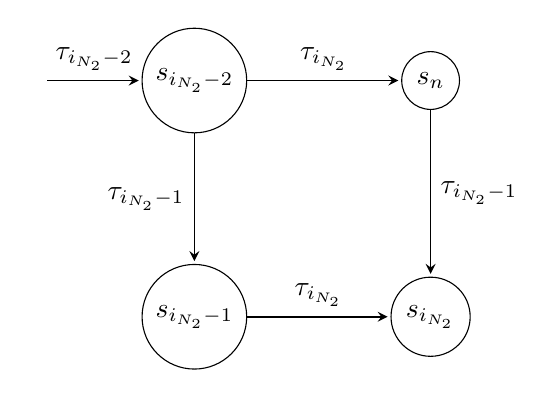
\begin{tikzpicture}
    [pre/.style={<-,shorten <=1pt,>=stealth,semithick}]
    \node (A) at (0,0) {};
    \node [shape=circle,draw=black] (B) at (2, 0) {\(s_{i_{N_2}-2}\)}
      edge [pre] node[above] {\(\tau_{i_{N_2}-2}\)} (A);
    \node [shape=circle,draw=black] (C) at (2, -3) {\(s_{i_{N_2}-1}\)}
      edge [pre] node[left] {\(\tau_{i_{N_2}-1}\)} (B);
    \node [shape=circle,draw=black] (D) at (5, 0) {\(s_{n}\)}
      edge [pre] node[above] {\(\tau_{i_{N_2}}\)} (B);
    \node [shape=circle,draw=black] (E) at (5, -3) {\(s_{i_{N_2}}\)}
      edge [pre] node[right] {\(\tau_{i_{N_2}-1}\)} (D)
      edge [pre] node[above] {\(\tau_{i_{N_2}}\)} (C);
  \end{tikzpicture}
  \caption{Commutativity Diagramm of Node scheduling}
\label{fig:chap3:sec_sync:commutativity_scheduling}
\end{figure}

\todo{The praragraph is a bit handwavy, needs more theory}
Figure~\ref{fig:chap3:sec_sync:commutativity_scheduling} visualizes how changing the order of the Nodes \(N_c, N_2\) has no influence on the global state after both have executed.
This follows from the fact, that both Nodes are independent of each other as shown before.
This means that the computation of one of them can't change the State of the other, thereby having absolutely no consequence on the computation of the other.
If both Nodes have mutual children, that children will receive their inputs in different order, but because the events are  on different channels it doesn't matter.
Therefore it doesn't matter which of the both Nodes is scheduled first: the state of the system will be different only at one position, but afterwards they both will have the same State again.
If one of the Nodes generate an output event, that event will be emitted one step earlier or later, which is also not relevant for the global State.

\todo{Here the induction step should happen, right?}


\subsection{Equality of synchronous and asynchronous schedules}
\label{sec:concepts:equalitys_without_timing:sync_async}

When the Nodes of \(A\) aren't scheduled in reversed topological order, the system can consume Inputs before producing all outputs based on the last consumed Input.
Therefore the reordering of runs has to be performed over wider parts of the run.
% Idea: each step is a commutation of two internal events in regard to the rev top order.
% => show commutativity of traces (note: only valid commutations, no two events, where one depends one the other, can be commuted, this is ensured by the scheduling of nodes that have input buffered)

\section{Behaviour with Timing functions}
\section{Equalitys with Timing functions}
section{Parallel computation}
